\documentclass{standalone}
\usepackage{graphicx}	
\usepackage{amssymb, amsmath}
\usepackage{color}

\usepackage{tikz}
\usetikzlibrary{intersections, backgrounds, patterns, patterns.meta}
\usepackage{pgfmath}

\definecolor{light}{RGB}{220, 188, 188}
\definecolor{mid}{RGB}{185, 124, 124}
\definecolor{dark}{RGB}{143, 39, 39}
\definecolor{highlight}{RGB}{180, 31, 180}
\definecolor{gray10}{gray}{0.1}
\definecolor{gray20}{gray}{0.2}
\definecolor{gray30}{gray}{0.3}
\definecolor{gray40}{gray}{0.4}
\definecolor{gray60}{gray}{0.6}
\definecolor{gray70}{gray}{0.7}
\definecolor{gray80}{gray}{0.8}
\definecolor{gray90}{gray}{0.9}
\definecolor{gray95}{gray}{0.95}

\begin{document}

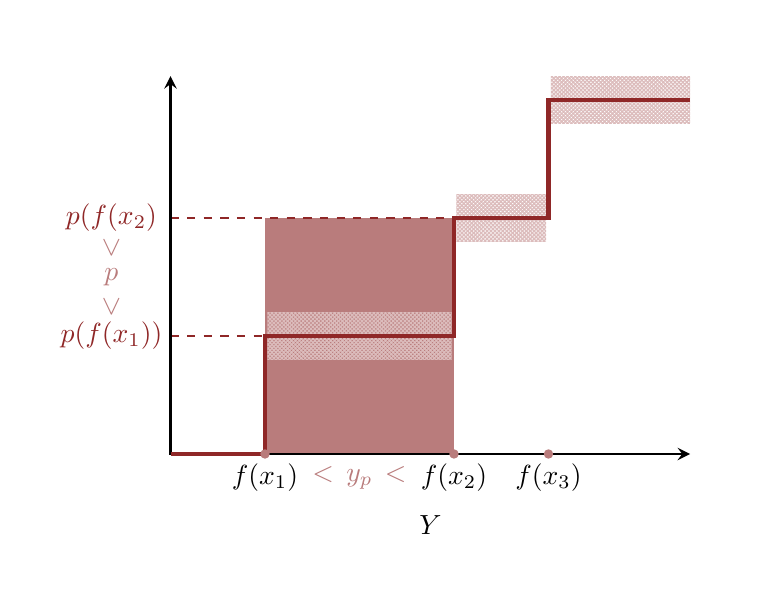
\begin{tikzpicture}[scale=0.3, thick]

\begin{scope}[shift={(0, 0)}]
  \draw[white] (-17, -5) rectangle (13, 18);

  %\draw[mid] (-11, 7.5) -- (1, 7.5);
  \node[mid] at (-13.5, 7.5) { $p$ };
  \node[mid] at (-3, -1) { $ < \, y_{p} \, < $ };
  
  \node[mid, rotate=90] at (-13.5, 8.75) { $<$ };
  \node[mid, rotate=90] at (-13.5, 6.25) { $<$ };
  
  \fill[mid] (-7, 0) rectangle (1, 10);

  \draw[dark, dashed] (-11, 5) -- (-7, 5);
  \node[dark] at (-13.5, 5) { $p(f(x_{1}))$ };

  \draw[dark, dashed] (-11, 10) -- (1, 10);
  \node[dark] at (-13.5, 10) { $p(f(x_{2})$ };
  
  \draw [->, >=stealth, line width=1] (-11, 0) -- (-11, 16);

  \draw [->, >=stealth, line width=1] (-11.05, 0) -- (11, 0);
  \node at (0, -3) { $Y$ };
  
  \fill[pattern={Hatch[angle=45,distance=1, line width=0.5]}, pattern color=light] 
    (-7 + 0.1, 4) rectangle (1 - 0.1, 6);

  \fill[pattern={Hatch[angle=45,distance=1, line width=0.5]}, pattern color=light] 
    (1 + 0.1, 9) rectangle (5 - 0.1, 11);
    
  \fill[pattern={Hatch[angle=45,distance=1, line width=0.5]}, pattern color=light] 
    (5 + 0.1, 14) rectangle (11, 16);
  
  \draw[dark, line width=1.5] (-11, 0) -- (-7, 0) -- (-7, 5) -- (1, 5) -- (1, 10) -- (5, 10) -- (5, 15) -- (11, 15);
 
  \fill[mid] (-7, 0) circle (0.2);
  \node at (-7, -1) { $f(x_{1})$ };
  
  \fill[mid] (1, 0) circle (0.2);
  \node at (1, -1) { $f(x_{2})$ };
  
  \fill[mid] (5, 0) circle (0.2);
  \node at (5, -1) { $f(x_{3})$ };
  
\end{scope}
  
\end{tikzpicture}

\end{document}  